%!TEX root = ../thesis.tex
%*******************************************************************************
%****************************** Optim2D Chapter ********************************
%*******************************************************************************
\chapter{L-BFGS Optimisation of Phase-Only Hologram}
\label{chapter:L-BFGS Optimisation of Phase-Only Hologram}

\graphicspath{{Chapter_Optim2D/Figs/}}


As previously introduced in \cref{chapter:Literature Review}, currently available spatial light modulators (SLMs) can only modulate either phase or amplitude, so algorithms are needed to compute amplitude-only or phase-only holograms, among which the phase-only holograms are usually preferred due to their higher energy efficiency, leading to the emergence of the classical phase retrieval algorithms reviewed in \cref{sec:cgh}. With the developments in modern numerical optimization methods and computational power, advances in CGH algorithms can be made. A search in the literature has found some recent work generating CGH using numerical optimisation methods \cite{Zhang2017, Liu2020, Choi2021, Chen2021}. This chapter therefore implements the use of numerical optimisation methods for hologram generation, including the novel method using the L-BFGS optimiser to compute phase-only holograms. The following sections start from the background knowledge of numerical optimization including L-BFGS algorithm, which also serves as the theoretical background for \cref{chapter:Multi-Depth Phase-Only Hologram Optimization} and \cref{chapter:Multi Frame Holograms Batched Optimization}, then introduces and carries out the optimization of phase hologram.



\section{Numerical Optimisation Methods} \label{sec:Numerical Optimisation Methods}

\subsection{Optimisation framework} \label{sec:Optimisation framework}
Numerical optimisation methods aim to find an optimal solution which minimise an objective function numerically. They begin with an initial guess of the optimal solution ($\textbf{x}_{0}$) and then, after iterations, generate a sequence of gradually improved estimates until they reach a solution \cite{Nocedal2006}. If we have $\textbf{x}$ as the vector of variables, and denote $f(\textbf{x})$ as the objective function, which is a function of $x$ we want to minimise, any unconstrained optimisation problem can be written as:
\begin{equation}
  \underset{\textbf{x}\in R^n}{\text{minimise}}\quad f(\textbf{x})
  \label{eq:minimise_F}
\end{equation}

Numerical optimisation then calculate the optimal solution $\textbf{x}^*$ iteratively, the iteration is given by:
\begin{equation}
  \textbf{x}_{k+1} = \textbf{x}_k+\alpha_k \textbf{p}_k
  \label{eq:optimisation_iteration}
\end{equation}
where the positive scalar $\alpha_k$ is called step length, or sometimes may be referred as `learning rate' in some context, and the vector $\textbf{p}_k$ is the search direction, which usually takes the form of
\begin{equation}
  \textbf{p}_k = -\textbf{B}_k^{-1} \nabla f_{k} \label{eq:general-descent-direction}
\end{equation}
where $\textbf{B}_k$ is a nonsingular matrix that varies for different optimisation methods, and $\nabla f_k$ is the gradient, which, if unable to evaluate directly, can be approximated by:
\begin{align}
  \nabla f_k         & \approx \frac{f_{k+1}-f_{k}}{\textbf{x}_{k+1}-\textbf{x}_{k}} \nonumber \\
  \text{where}\  f_k & \ \text{denotes}\  f(\textbf{x}_k)
\end{align}

The strategy used to determine $\textbf{p}_k$ distinguishes one algorithm from another. Most methods make use of the values of $f$, $\nabla f$ and $\nabla^2 f$, and some methods even make use of the accumulated historical values of those derivatives, which are further discussed in \cref{sec:GD} - \cref{sec:L-BFGS}.


\subsection{Gradient Descent}\label{sec:GD}
Gradient descent (GD) is a first-order optimisation method, it finds a local minimum by following the negative of the gradient (i.e. the steepest descent direction). The $\textbf{B}_k$ (in \cref{eq:general-descent-direction}) for gradient descent simply takes the value of $\textbf{I}$, which is the identity matrix. And the search direction becomes:
\begin{equation}
  \textbf{p}_k = -\nabla f_k
\end{equation}
The steepest descent method is very intuitive: among all possible directions to move away from $\textbf{x}_{k}$, the steepest gradient direction is the one which $f$ decreases most rapidly. The advantage of this method is that it requires few computation and memory resource, because it only requires a computation of the first derivative, and it does not require any accumulation of historical gradients. However, it is a greedy method that only considers the current iteration without any global consideration, so it can be extremely slow on complicated problems. \cite{Nocedal2006}

To work around the disadvantage, a few variants have emerged, such as AdaGrad \cite{Duchi2011}, RMSProp \cite{Tieleman2012} and Adam \cite{Kingma2015} which combines the advantages of AdaGrad and RMSProp. The Adam method is an iconic variant of GD, often referred to as `gradient descent with momentum', as the name Adam is derived from `adaptive moment estimation'. Adam algorithm is based on adaptive estimates of lower-order moments \cite{Kingma2015}. It computes individual adaptive learning rates for different parameters from estimates of first and second moments of the gradients \cite{Kingma2015}.


\subsection{Newton's Method}
Newton's method is a second-order optimisation method. Its search direction is derived from the second-order Taylor series approximation to $f(\textbf{x}_k+\textbf{p})$, which is
\begin{equation}
  f(\textbf{x}_k+\textbf{p}) \approx f_k + \textbf{p}^T \nabla f_k + \frac{1}{2}\textbf{p}^T \nabla^2 f_k \textbf{p} \stackrel{\text{def}}{=}m_k(\textbf{p})
\end{equation}
The Newton direction can then be obtained by finding the vector $\textbf{p}$ that minimises $m_k(\textbf{p})$. By setting the derivative of $m_k(\textbf{p})$ to zero, $\textbf{p}$ can be obtained as:
\begin{equation}
  \textbf{p}_k=-\nabla^2 f_k^{-1}\nabla f_k \label{eq:Newton-direction}
\end{equation}
By comparing \cref{eq:Newton-direction} to \cref{eq:general-descent-direction}, it can be seen that the Newton's method has a $\textbf{B}_k$ of $\nabla^2 f_k$. Unlike the gradient descent method, there is a "natural" step length of 1 associated with the Newton direction, so $\alpha_k = 1$ by default and is only adjusted when it does not produce a satisfactory reduction in the value of $f$.

The Newton direction is reliable when the difference between the true function $f(\textbf{x}_k+\textbf{p})$ and its quadratic model $m_k(\textbf{p})$ is not too large. Methods that use the Newton direction have a fast rate of local convergence, typically quadratic. After a neighbourhood of the solution is reached, convergence to high accuracy often occurs in just a few iterations. The main drawback of the Newton direction is the need for the Hessian $\nabla^2 f_k$. Explicit computation of this matrix of second derivatives can sometimes be a cumbersome, error-prone, and expensive process. \cite{Nocedal2006}


\subsection{Quasi-Newton Method}\label{sec:BFGS}
Quasi-Newton method provides an attractive alternative to Newton's method, in that they do not require computation of the Hessian and yet still attain a super linear rate of convergence. In place of the true Hessian $\nabla^2 f_k$, they use an approximation $\mathcal{H}_k \stackrel{\text{def}}{=} \textbf{B}_k^{-1}$, which is updated after each step to take account of the additional knowledge gained during the step. The updates make use of the fact that changes in the gradient provide information about the second derivative of $f$ along the search direction. The most popular quasi-Newton algorithm is the Broyden-Fletcher-Goldfarb-Shanno (BFGS) method, named for its discoverers Broyden, Fletcher, Goldfarb, and Shanno. \cite{Nocedal2006}

The process of the BFGS method is shown below:
\begin{align}
  denote   & \                       \left\{
  \begin{array}{ll}
    \mathcal{H}_k & = \textbf{B}_k^{-1}          \\
    \textbf{p}_k & = -\mathcal{H}_k \nabla f_{k}
  \end{array}
  \right.                                                                                                                                                                                                        \\
  Initiate & \ \mathcal{H}_0     \leftarrow \frac{\textbf{y}_k^T\textbf{s}_k}{\textbf{y}_k^T\textbf{y}_k}\textbf{I}                                                           \label{eq:BFGS_initiate_H_0}        \\
  update   & \ \mathcal{H}_{k+1}  = (\textbf{I} - \rho_k\textbf{s}_k\textbf{y}_k^T) \mathcal{H}_{k} (\textbf{I} - \rho_k\textbf{y}_k\textbf{s}_k^T) +\rho_k\textbf{s}_k\textbf{s}_k^T \label{eq:BFGS_update_H_k+1} \\
  where    & \                        \left\{
  \begin{array}{ll}
    \textbf{s}_k & = \textbf{x}_{k+1} - \textbf{x}_{k}                               \\
    \textbf{y}_k & = \nabla f_{k+1} - \nabla f_{k}                                   \\
    \rho_k       & = \frac{1}{\textbf{y}_k^T\textbf{s}_k} \label{eq:BFGS_calc_rho_k}
  \end{array}
  \right.
\end{align}

The algorithm is robust, and its rate of convergence is super linear, which is fast enough for most practical purposes. Even though Newton's method converges more rapidly (that is, quadratically), its cost per iteration usually is higher, because of its need for second derivatives and solution of a linear system. The drawback is that, it is not directly applicable to large optimisation problems because $\mathcal{H}_k$'s are usually dense, requiring large storage and computational requirements. \cite{Nocedal2006}


\subsection{Large Scale Quasi-Newton Method: Limited Memory BFGS (L-BFGS)}\label{sec:L-BFGS}
L-BFGS algorithm \cite{Liu1989} modifies the technique described in \cref{sec:BFGS} to obtain Hessian approximations that can be stored compactly in just a few vectors of length $n$, where $n$ is the number of unknowns in the problem. The main idea of this method is to use curvature information from only the most recent iterations to construct the Hessian approximation. Curvature information from earlier iterations, which is less likely to be relevant to the actual behaviour of the Hessian at the current iteration, is discarded in the interest of saving storage. \cite{Nocedal2006}

Denoting $\textbf{V}_k = \textbf{I} - \rho_k\textbf{y}_k\textbf{s}_k^T$, \cref{eq:BFGS_update_H_k+1} can be written as:
\begin{equation}
  \mathcal{H}_{k+1} = \textbf{V}_k^T \mathcal{H}_{k} \textbf{V}_k +\rho_k\textbf{s}_k\textbf{s}_k^T
\end{equation}

The inverse Hessian approximation $\mathcal{H}_{k}$ will generally be dense, so that the cost of storing and manipulating it is prohibitive when the number of variables is large. To circumvent this problem, we store a modified version of $\mathcal{H}_{k}$ implicitly, by storing a certain number (say, $m$) of the vector pairs $\{\textbf{s}_i, \textbf{y}_i\}$ used in the \cref{eq:BFGS_update_H_k+1} and \cref{eq:BFGS_calc_rho_k}. The product $\mathcal{H}_{k} \nabla f_k$ can be obtained by performing a sequence of inner products and vector summations involving $\nabla f_k$ and the pairs $\{\textbf{s}_i, \textbf{y}_i\}$. After the new iterate is computed, the oldest vector pair in the set of pairs $\{\textbf{s}_i, \textbf{y}_i\}$ is replaced by the new pair $\{\textbf{s}_k, \textbf{y}_k\}$ obtained from the current step (\cref{eq:BFGS_calc_rho_k}). In this way, the set of vector pairs includes curvature information from the $m$ most recent iterations. Practical experience has shown that modest values of $m$ (between 3 and 20, say) often produce satisfactory results. We now describe the updating process in a little more detail. At iteration $k$, the current iterate is $\textbf{x}_k$ and the set of vector pairs is given by $\{\textbf{s}_i, \textbf{y}_i\}$ for $i=k-m,\ldots,k-1$. We first choose some initial Hessian approximation $\mathcal{H}_{k}^0$ (in contrast to the standard BFGS iteration, this initial approximation is allowed to vary from iteration to iteration) and find by repeated application of \cref{eq:BFGS_update_H_k+1} that the L-BFGS approximation $\mathcal{H}_{k}$ satisfies the following formula: \cite{Nocedal2006}

\begin{align}
  \mathcal{H}_{k} =\  & (\textbf{V}_{k-1}^T \cdots \textbf{V}_{k-m}^T) \mathcal{H}_{k}^0 (\textbf{V}_{k-m} \cdots \textbf{V}_{k-1})                                  \nonumber          \\
                     & + \rho_{k-m} (\textbf{V}_{k-1}^T \cdots \textbf{V}_{k-m+1}^T) \textbf{s}_{k-m} \textbf{s}_{k-m}^T (\textbf{V}_{k-m+1} \cdots \textbf{V}_{k-1}) \nonumber       \\
                     & + \rho_{k-m+1} (\textbf{V}_{k-1}^T \cdots \textbf{V}_{k-m+2}^T) \textbf{s}_{k-m+1} \textbf{s}_{k-m+1}^T (\textbf{V}_{k-m+2} \cdots \textbf{V}_{k-1}) \nonumber \\
                     & + \cdots \nonumber                                                                                                                                             \\
                     & + \rho_{k-1} \textbf{s}_{k-1} \textbf{s}_{k-1}^T
\end{align}

From this expression we can derive a recursive procedure (\cref{alg:L-BFGS}) to compute the product $\mathcal{H}_{k} \nabla f_k$ efficiently.

\begin{algorithm}[H]
  \caption{L-BFGS two-loop recursion \cite{Nocedal2006}}\label{alg:L-BFGS}
  \begin{algorithmic}
    \State $\textbf{q} \gets \nabla f_k$
    \For{$i = k-1, k-2, ..., k-m$}
    \State $\alpha_i \gets \rho_i \textbf{s}_i^T \textbf{q}$
    \State $ \textbf{q} \gets \textbf{q} - \alpha_i\textbf{y}_i$
    \EndFor
    \State $\textbf{r}\gets \mathcal{H}_k^0 \textbf{q}$
    \For{$i = k-m, k-m+1, ..., k-1$}
    \State $\beta \gets \rho_i \textbf{y}_i^T \textbf{r}$
    \State $ \textbf{r} \gets \textbf{r} +\textbf{s}_i (\alpha_i-\beta)$
    \EndFor
    \State Step with $\textbf{p}_k \gets -\mathcal{H}_k \nabla f_{k} = -\textbf{r}$
  \end{algorithmic}
\end{algorithm}

Apart from being inexpensive, L-BFGS has the advantage that the multiplication by the initial matrix $\mathcal{H}_k^0$ is isolated from the rest of the computations, allowing this matrix to be chosen freely and to vary between iterations. A method for choosing $\mathcal{H}_k^0$ that has proved effective in practice is to use the same as BFGS as stated in \cref{eq:BFGS_initiate_H_0}. \cite{Nocedal2006}


\section{Implementation of Optimisation Methods on CGH}

To implement the optimisation methods listed in \cref{sec:Numerical Optimisation Methods} on CGH, firstly the optimisation framework needs to be adapted. The objective is to find the phase hologram (H) that has the optimal reconstruction (R) matching the target image (T), which can be formulated as minimising the difference between R and T by varying H, leading to the mathematical expression:
\begin{equation}
	\underset{\textbf{H}}{\arg \min}\ Loss(\textbf{T}, \textbf{R})
\end{equation}
where $Loss$ denotes a loss function quantifying the difference between T and R, and $\arg$ returns the argument (H) of the optimisation. There are

The phase-only constraint of CGH can be easily applied by fixing a constant amplitude of the hologram, while keeping its phase varying and being the argument of optimization ($\textbf{x}$).

\begin{figure}[H]
	\centering
	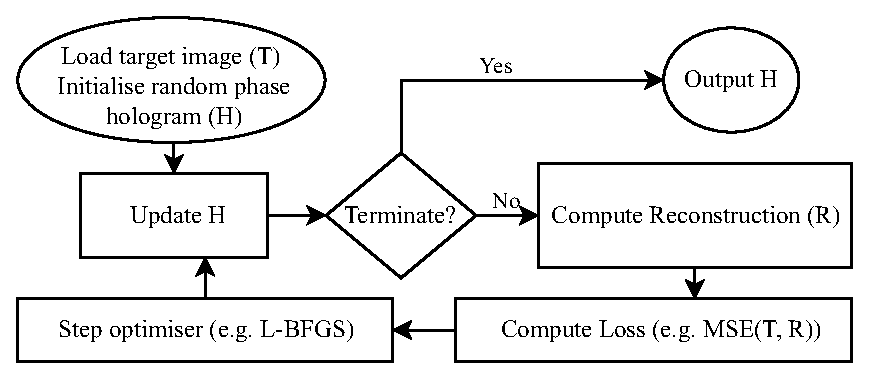
\includegraphics[width=\textwidth]{optim_flowchart_2D.eps}
	\caption{Flowchart of the optimisation process}
	\label{fig:optim_flowchart_2D}
\end{figure}

\begin{equation}
  MSE(\textbf{T}, \textbf{R}) = \frac{1}{X\times Y} \sum_{x=1}^{X} \sum_{y=1}^{Y} (\textbf{T}_{x,y}-\textbf{R}_{x,y})^2
\end{equation}

\begin{figure}[H]
	\centering
	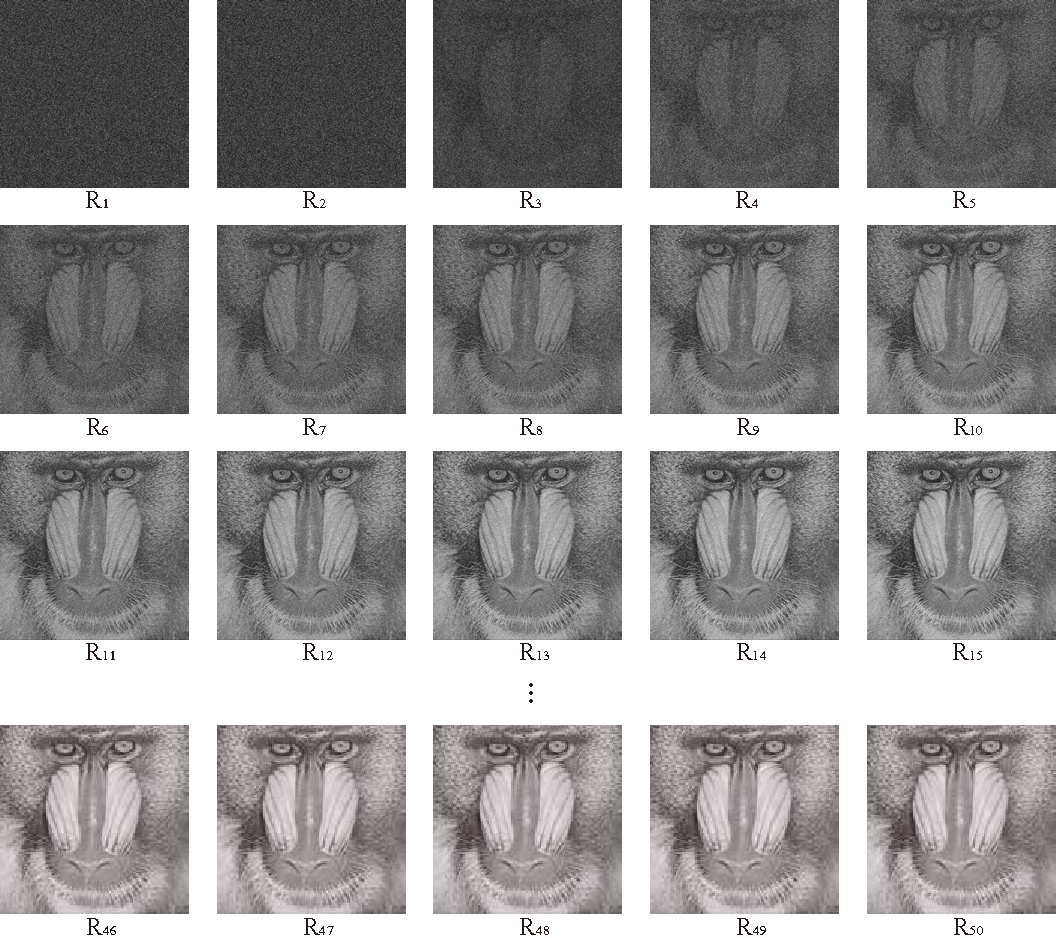
\includegraphics[width=\textwidth]{LBFGS_iters.pdf}
	\caption{Reconstructions at the first 20 iterations of the L-BFGS optimisation}
	\label{fig:LBFGS_iters}
\end{figure}

\begin{figure}[H]
	\centering
	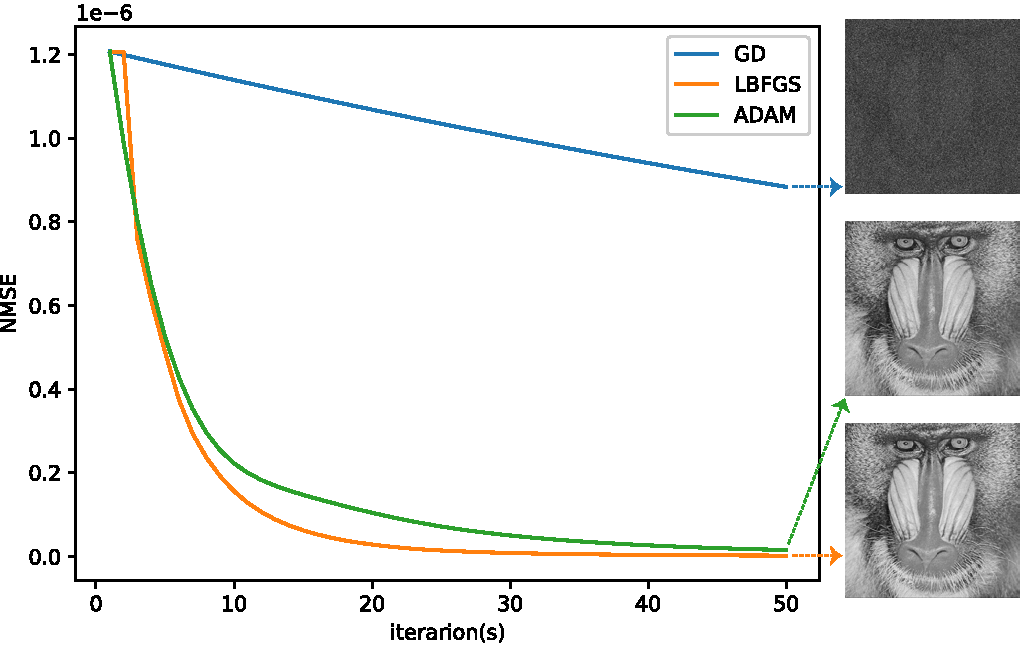
\includegraphics[width=\textwidth]{GD_ADAM_LBFGS.pdf}
	\caption{Convergence plot for comparison between the GD, Adam and L-BFGS optimisations}
	\label{fig:GD_ADAM_LBFGS}
\end{figure}

